\section{Introduction and Motivation}\label{sec:introduction}
In the era of Information Technology, the usage of software and its applications is continuously increasing and has become an important part of our lives. This makes the software industry one of the largest industries in the world and many companies are built around the development of software. With the growing usage of software, the software development process has changed drastically and has become more solution-oriented. Nowadays, the entire focus is on making the software development process fast, less complex, and more human-friendly. 

One of the approaches to reducing the complexity of software development is abstraction and separation of concerns~\cite{modeltransform}. In recent times, (software) modeling has become an effective way of implementing this principle. In a traditional approach, developers manually write programs and check the specifications, which is often costly, incomplete, informal, and carries a major risk of failure. In contrast, model-driven software development (referred to as \textbf{MDSD} from now on) improves the way software is built by moving the focus from code to representing the essential aspects of software in the form of software models. It reduces development costs and increases the reusability and maintainability of software. The objective of MDSD~\cite{modeltransform} is to increase productivity and reduce time-to-market by enabling development at a higher level of abstraction and by using concepts closer to the problem domain, rather than what is directly offered by programming languages.
 
The core idea of the MDSD approach is based on models, modeling and model transformations. In this approach, developers represent real world systems as models at a suitable level of abstraction. Different models can be used to represent different views of a system.  Although these views are separate and result in models that can be independently manipulated by different developers, there are still numerous relations between models that must be taken into account to ensure that the entire system, described by the state of all models, is consistent. This can be handled by model transformation to increase the developers' productivity and quality of the models.

\textit{Bidirectional transformation} (referred to as \textbf{bx} from now on) is a technique used to synchronize two (or more) models. Such models are related, but don't necessarily contain the same information. Changes in one model can thus lead to changes in other models \cite{bx-grace}.
\newline\newline\textit{Bidirectional transformation} is used to deal with scenarios like~\cite{bx-theoryandappl}:\\

\begin{itemize}
	\item {change propagation to the user interface as a result of underlying data changes}	
	\item {synchronization of business/software models}
	\item {refreshable data-cache incase of database changes}
	\item {consistency management between two artifacts by avoiding data loss}
\end{itemize}

The bx community (\url{http://bx-community.wikidot.com/}) has been doing research in many fields including software development, databases, mathematics and much more, to increase awareness for bx ~\cite{bx-grace}\cite{bx-dagstuhl}. As a result, many kinds of bx tools are being developed. These bx tools are based on various approaches, such as graph transformations e.g., eMoflon~\cite{emoflon-part4}, bidirectionalization e.g., BIGUL~\cite{bigul}, constraint solving e.g., Echo~\cite{echo} and can be used in different areas of application~\cite{bx-community}.

\subsection{Problem Statement}\label{subsec:probstmt}
\textit{Bidirectional transformation} is an emerging concept. In the past, many efforts have been made by conducting international workshops, seminars and through experiments conducted by developers / bx community to identify its potential. Also, in addition to the development of bx tools and bx language, benchmarks are being created for bx tools for systematic comparison~\cite{benchmark-BX}.

Although a significant amount of work has been done on bx, a general awareness and understanding for basic concepts, the involved challenges, and reasonable expectations is not really given. Hence, there exist conceptual and practical challenges with building software systems using bx-tools and as a result bx tools and their applicability is still not widely known and used~\cite{bx-theoryandappl}.

From experience with working with master students (future software developers) and bx researchers, we have identified that imparting knowledge about certain core bx concepts can improve the situation. However, the problem is that it is relatively hard and challenging to do this as current possibilities (virtual machines, handbooks, etc) are either tool specific or ineffective because installation process to get the tool running is a time consuming process and sometimes requires technical expertise in a specific area/tool/programming language. Even after you get the tool running, it doesn't necessarily help in understanding bx concepts because of lack of proper explanations. Just examples are not interactive enough, anything tool-specific gets into too much detail of the respective tool, etc.  So a platform on which one can easily prepare high-quality, easily understandable, and engaging learning material for spreading the bx concepts is missing.

To keep a focus on the above described problem statements and to relate to the work done directly or indirectly during my entire thesis, I have formulated the following associated research questions (referred to as \textbf{RQ} from now on):

\begin{itemize}
	\item {\textbf{\textit{RQ1}} -- What are the core requirements for implementing a successful bx demonstrator ?}
	\item {\textbf{\textit{RQ2}} -- Which goals can be particularly well addressed in a bx demonstrator and why ?}
	\item {\textbf{\textit{RQ3}} -- Is it possible to teach the concepts of bx through a demonstrator ?}
	\item {\textbf{\textit{RQ4}} -- Does an interactive GUI helps an user to increase his/her understanding of bx concepts ?}
\end{itemize}

\subsection{Contribution}\label{subsec:contribution}
To solve the problems as described in Section \ref{subsec:probstmt}, in this thesis, my goals are as follows:
\begin{itemize} 
\item {Design and implement an interactive demonstrator.} 
\item {Spread the basic concepts of bx to a wide audience and making them accessible and understandable.}
\end{itemize}

An existing bx tool will be used as a part of the demonstrator to realize \textit{bidirectional transformation}. The final prototype will be interactive and easily accessible to users to help them understand the potential, power and limitations of bx.

My contribution towards providing a solution to the problems described in Section \ref{subsec:probstmt}  can be categorised into three parts as shown in Figure~\ref{fig:Contribution}. 

\begin{figure}
	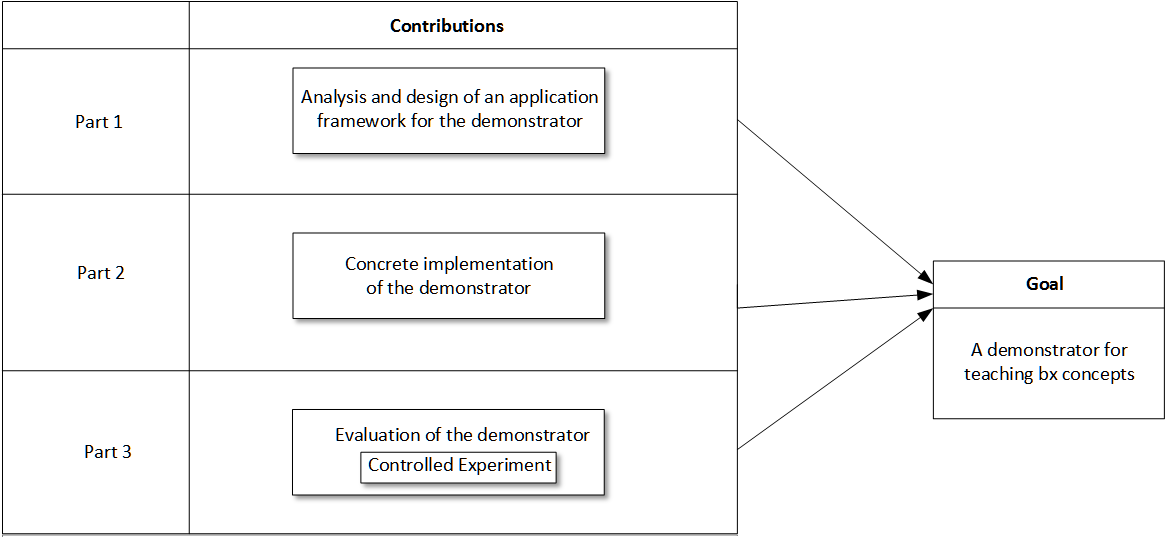
\includegraphics[width=1\textwidth]{figures/Contribution}
	\caption{Contributions}
	\label{fig:Contribution}
\end{figure}

\paragraph{Contribution 1: Analysis and Design}
First, I analyzed the already existing work on bx and find out the related problems. Detail explanation of all my findings are described in Section \ref{sec:relatedwork}. Then by considering the problems in hand, I have designed a working, fully functional application framework based on MVC pattern for implemenating a bx tool demonstartor along with a interactive user interface. Section \ref{sec:design_model} explains the design process in detail. This framework can be used to implement a demonstrator encapsulating a bx tool with a concrete example.

\paragraph{Contribution 2: Concrete Implementation}
Secondly, I have implemented a fully functional demonstrator based on the application framework designed earlier. This demonstrator is based on a bx tool i.e., eMoflon 
\newline\newline First, I have constructed a few examples which can be implemented covering the requirements and showing the usability of bx tools through demonstrator. Then, taking account the availabilities of resources and usability factor, I finally chose the best suitable example to implement and build the final prototype. Section \ref{subsec:exampleforimplementation} describes list of all the examples.
\newline\newline Second step was to choose a bx-tool for my demonstrator. Based on the gathered information and taking account implementation related issues, I have chosen a bx-tool to be used as a part of the demonstrator to realize bx. Section \ref{subsec:bxtoolselection} explains the process in detail.
\newline\newline Next step was to set up the entire application framework for implementing the demonstrator. First, I did some research by going through materials on software design patterns and web application architecture. Then, I prepared a few proof of concepts(POC) for checking the feasibilty of the architecture designs before finalising my application framework. Section \ref{subsec:architecturedesign} explains the process in detail.

\paragraph{Contribution 3: Evaluation} 
This stage is based on the research method called Controlled Experiments \cite{semethods}. This experiment is based on one or more hypothesis, which guide all steps of the experimental design, deciding which variables to include and how to measure them. So, it is an investigation of one or more hypothesis where one or more independent variables are manipulated to measure their effect on one or more dependent variables. Learning goals were prepared along with the scenarios to explain them and questions were asked on these concepts to different groups of participants. Finally, data is collected and analyzed to measure the outcome. Section \ref{sec:evaluation} explains the process in detail.

\subsection{Structure of Thesis}\label{subsec:structure}

Chapter 1 (introduction) contains the introduction and motivation about the thesis with a solution strategy. Chapter 2 discusses the related terminologies with respect to bidirectional transformation. Chapter 3 describes the requirements for implementing a successful bx demonstrator. Chapter 4 explains the related work that has been done on bx in last few years and their related problems. Chapter 5 describes all the design decisions and its associated challenges during the implementation work. Chapter 6 provides in-depth explaination of the implementation details done in each layer along with UML diagrams. Chapter 7 contains the learning goals (based on research questions), feedback from user groups, and evaluation results. Last chapter summarizes all the work which was done as part of this thesis and draws conclusions followed by future work.

\clearpage
\section{Foundation}\label{sec:foundation}
This chapter provides an overview of my running example in Section \ref{subsec:runningexample} followed by definitions of some commonly used terminologies with respect to bx in Section \ref{subsec:definitions}. This chapter will lay the foundation for understanding the basics for the reader and will help him/her in apprehending the concepts explained in further chapters.

In this thesis, bidirectional transformation will be discussed by referring to a \textit{Kitchen Model} and a \textit{Grid Model} of a software system. Both models describe the structure and behaviour of the real system "kitchen" but from different perspectives.

\subsection{Running Example}\label{subsec:runningexample}
This example is a simplified kitchen planner. Figure~\ref{fig:Running_Example_GUI} describes the relation between the \textit{Kitchen Model} denoted by \textit{Kitchen} (right-hand side canvas) and the \textit{Grid Model} denoted by \textit{Layout} (left-hand side canvas). 

\begin{figure}
	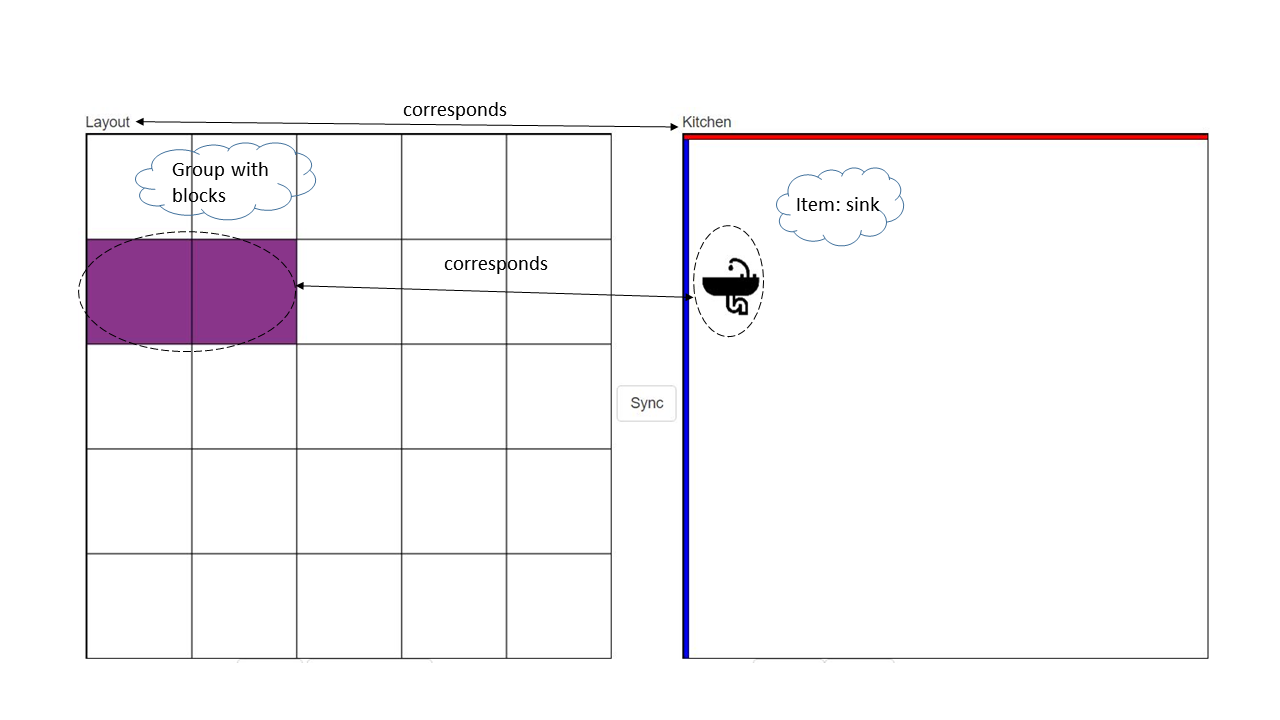
\includegraphics[width=1\textwidth]{figures/KitchenToGrid}
	\caption{Running Example: Layout and Kitchen}
	\label{fig:Running_Example_GUI}
\end{figure} 

\begin{figure}
	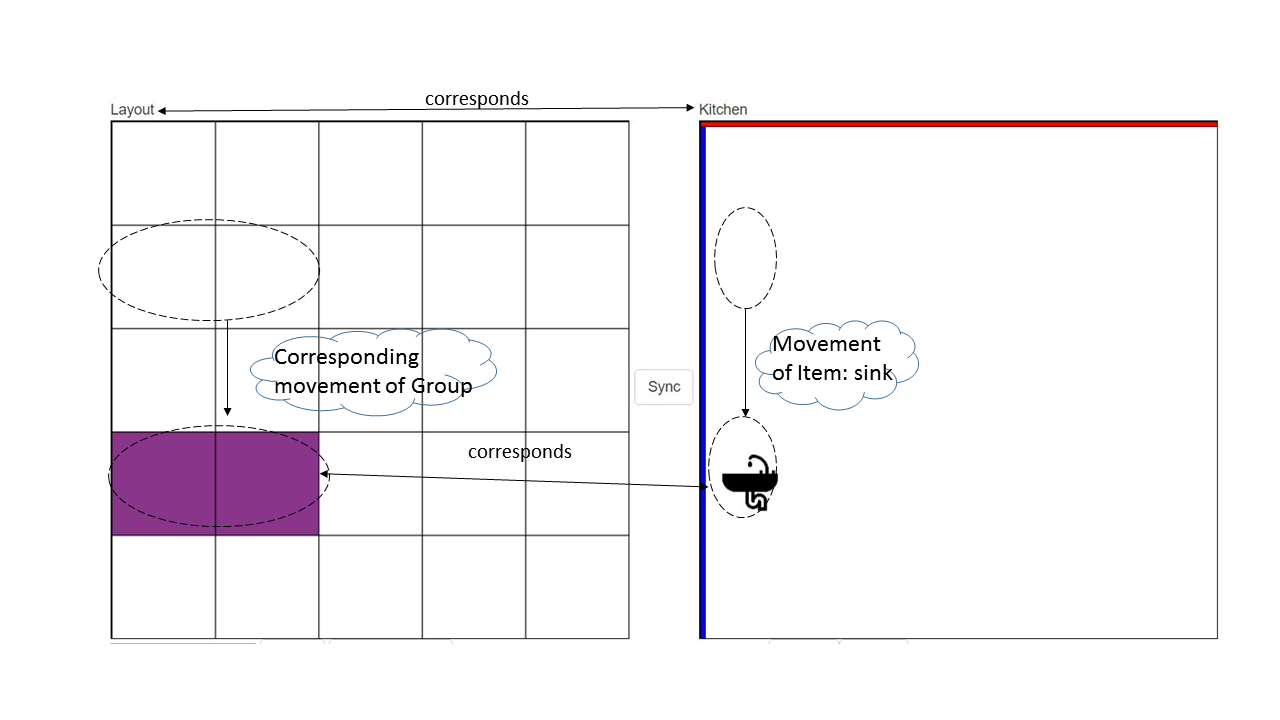
\includegraphics[width=1\textwidth]{figures/KitchenToGrid_consistency}
	\caption{Running Example: Consistency Preservation}
	\label{fig:Running_Example_GUI_consistency}
\end{figure}

\textit{Kitchen} contains items e.g., sink, fridge, table etc. You can create, delete or move these items in the kitchen, and press "Sync" to propagate your changes to the layout. The \textit{Layout} consist of groups with certain number of blocks. This shows how much space the objects occupy as coloured groups of blocks organised in a grid. Here, the \textit{Kitchen} corresponds to the \textit{Layout} and a single \textit{Item} corresponds to a \textit{Group}. This is described by Figure~\ref{fig:Running_Example_GUI} where an item e.g., \textit{sink} created in the \textit{Kitchen} corresponds to a group in the \textit{Layout}.

Both artifacts are created and evolve together during the lifecycle of the application representing a kitchen workspace. Thus, changes in one domain should be propagated to the other domain in order to ensure consistency between these related artifacts. This is shown by Figure~\ref{fig:Running_Example_GUI_consistency}.

Model transformation and synchronization is discussed with this scenario throughout this thesis. 

\subsection{BX Basics}\label{subsec:definitions}

\begin{defn}\label{defModel} (Model and Meta-Model)\\
A model depicts the structure and/or behavior of a real system under discussion from a certain point of view and at a certain level of abstraction which helps in managing and understanding the complexities of a system \cite{uml} \cite{mdsd}. Model creation helps in keeping a clear focus on selected concepts and rules relevant for a particular concern and omitting irrelevant details.

A metamodel describes a set of models, i.e., defines a modelling language. 
\end{defn} 

\begin{table}
	\centering	
	\begin{tabular}{|p{3cm}|p{3cm}|p{9cm}|}
		\hline
		\rowcolor[gray]{.8}	
		\textbf{Reality} & \textbf{Model} & \textbf{Aspects Covered} \\
		\hline
		Kitchen & Kitchen Model & 
		\begin{itemize}
			\item Area of a kitchen as a white space
			\item 4 walls of a kitchen
			\item Contains the objects of a kitchen
			\item Creation, movement, deletion of kitchen objects
		\end{itemize}\\
		\hline
		Kitchen & Grid Model & 
		\begin{itemize}
			\item Area of a kitchen as a block structure
			\item 4 walls of a kitchen
			\item Contains the objects of a kitchen
			\item Creation, deletion of kitchen objects
		\end{itemize}\\
		\hline					
		
	\end{tabular}
	\caption{Model and Reality}
	\label{tab:Model_Reality}
\end{table}

\textit{Example:} In my demonstrator, the example that I have two meta-models i.e., \textit{Kitchen} and \textit{Grid}. Both the models represent the reality "Kitchen". A relation between reality and models is shown in Table~\ref{tab:Model_Reality}. 

Figure~\ref{fig:Kitchen_MetaModel} depicts the \textit{Kitchen} meta-model as a class diagram from an object oriented point of view.

Figure~\ref{fig:Kitchen_AbstractConcrete} illustrates an abstract and concrete view of the \textit{Kitchen} model. Left-side figure shows an abstract syntax i.e., an instance of the kitchen. Whereas, right-side figure describes a concrete syntax of the kitchen as visualized in the user interface.\\

\begin{figure}
	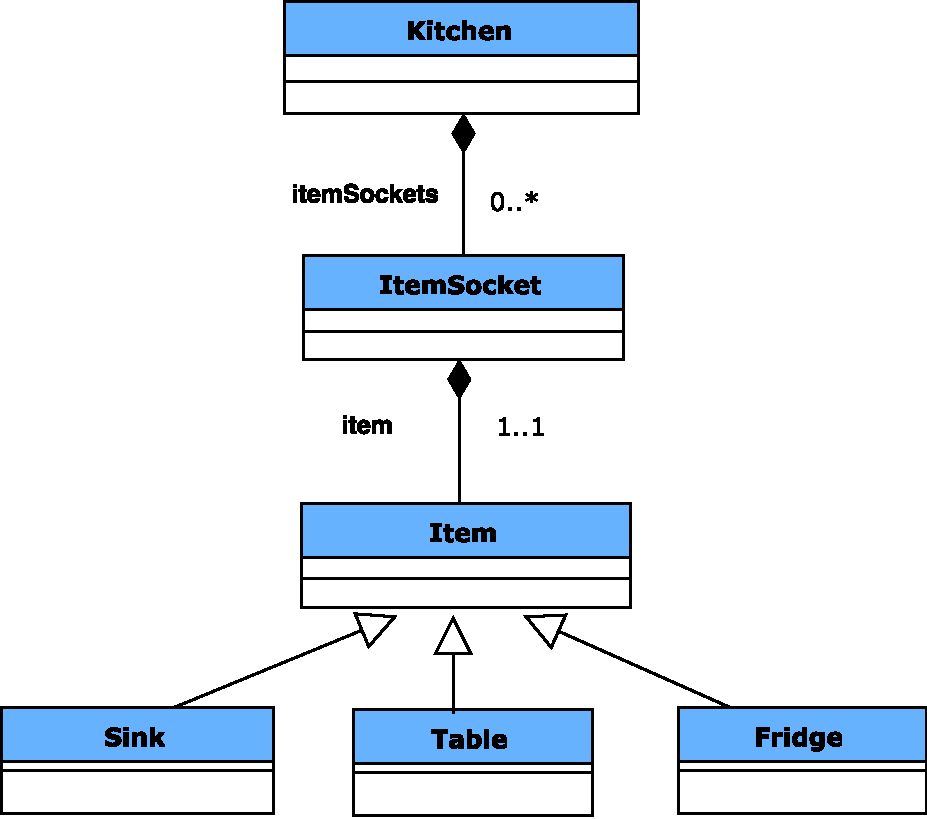
\includegraphics[width=0.7\textwidth]{figures/Kitchen_MetaModel}
	\caption{Kitchen Meta-Model}
	\label{fig:Kitchen_MetaModel}
\end{figure}

\begin{figure}
	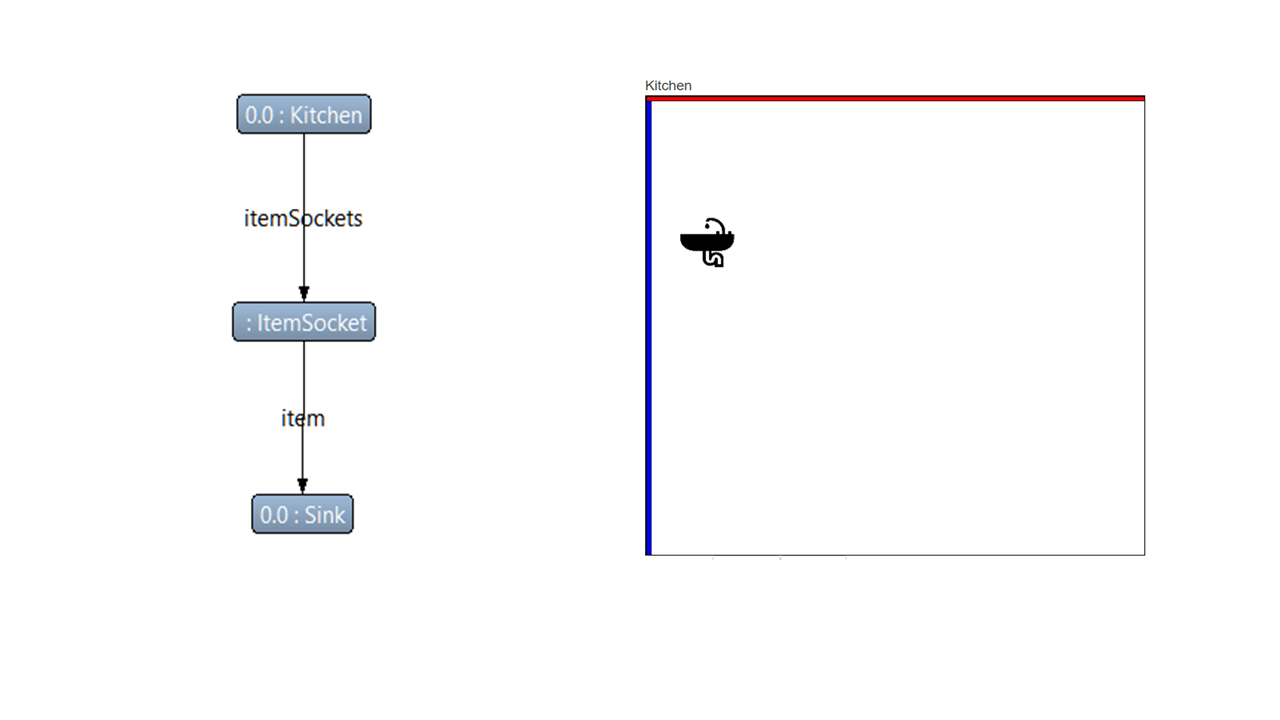
\includegraphics[width=1\textwidth]{figures/Kitchen_AbstractConcrete}
	\caption{Kitchen Model (Abstract \& Concrete)}
	\label{fig:Kitchen_AbstractConcrete}
\end{figure}

\begin{defn}\label{defDelta} (Delta)\\
A delta is the change applied to one or more properties of an artefact. It denotes the relationships between models from the same model space \cite{benchmarx-reload}. It is denoted $\delta$: M $\longrightarrow$ M' where M' is an updated version of M.
\end{defn}

\textit{Example:} In my demonstrator example, deltas related to the "Kitchen Model" are described in Table~\ref{tab:Examples_of_Delta}. Whereas, Figure~\ref{fig:Delta_Propagation} shows a concrete example of delta propagation, where creation of a new item e.g., sink causes the change from Kitchen to Kitchen'.\\

\begin{table}
	\centering	
	\begin{tabular}{|p{5cm}|p{10cm}|}
		\hline
		\rowcolor[gray]{.8}	
		\textbf{Model} & \textbf{Delta ($\delta$)} \\
		\hline
		Kitchen Model & 
		\begin{itemize}
			\item Creating a new item
			\item Deleting an existing item
			\item Moving an item
		\end{itemize}\\
		\hline				
		
	\end{tabular}
	\caption{Examples of Delta in Kitchen Model}
	\label{tab:Examples_of_Delta}
\end{table}

\begin{figure}
	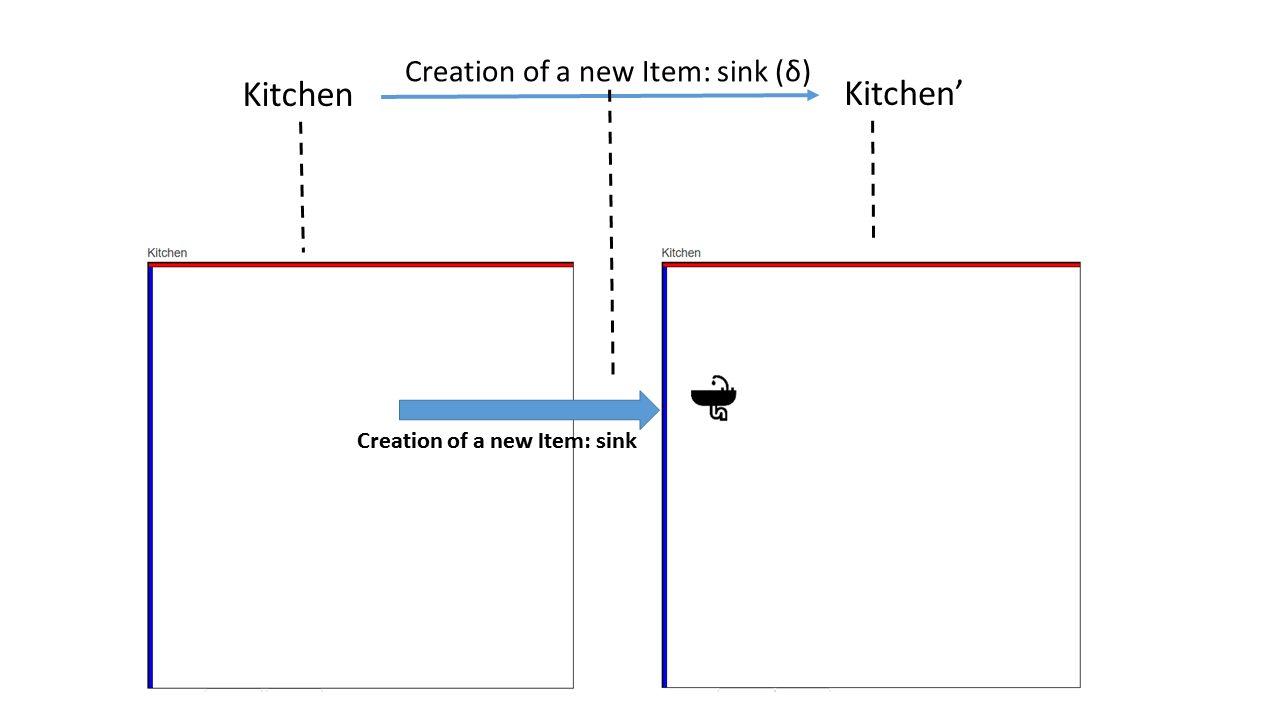
\includegraphics[width=1\textwidth]{figures/Delta_Propagation}
	\caption{Delta Propagation}
	\label{fig:Delta_Propagation}
\end{figure}

\begin{defn}\label{defModelSpace } (Model Space)\\
A Model Space describes all the states of an artefact (models) and all the deltas which lead from one model to another.
\end{defn}

\textit{Example:} In my demonstrator example, a concrete example of a subset of a model space is shown in Figure~\ref{fig:Model_Space} with the states i.e., Kitchen1, Kitchen2, Kitchen3, Kitchen4 along with deltas i.e., $\delta$1, $\delta$2, $\delta$3 of the \textit{Kitchen} Model.\\\\

\begin{figure}
	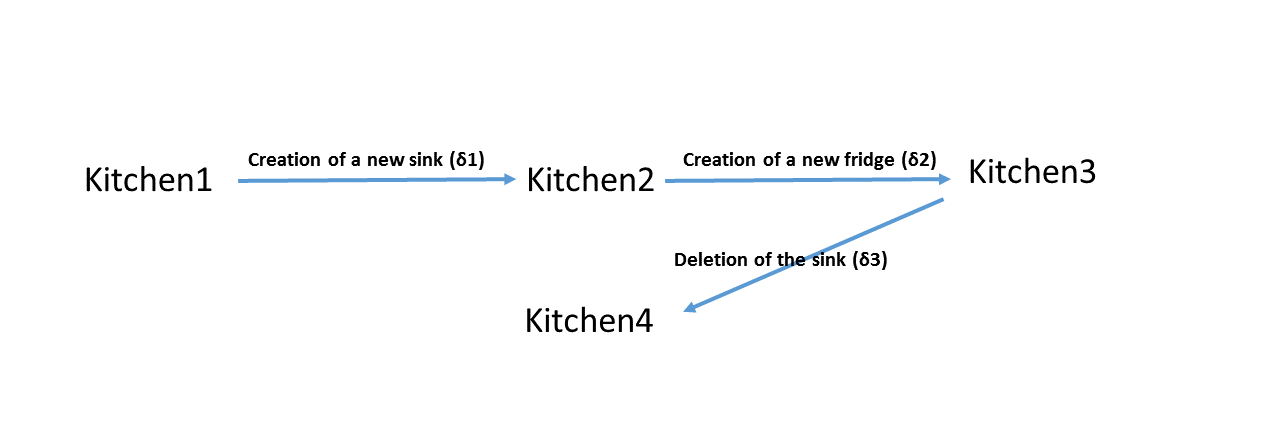
\includegraphics[width=1\textwidth]{figures/Model_Space}
	\caption{Model Space}
	\label{fig:Model_Space}
\end{figure}

\begin{defn}\label{defCorrespondenceLinks } (Correspondence Links)\\
Relationships between models from different model spaces are called correspondence links, or just corrs \cite{benchmarx-reload}. A corr is a set of links  r(a; b) between elements (a in A, b in B), which are compatible with the models' structure and denoted by double bidirectional arrows, e.g., R: A $\Longleftrightarrow$ B. 
\end{defn}

\textit{Example:} In my demonstrator example, an example of a corr is r(group; itemSocket) where \textit{group}, \textit{itemSocket} are the elements of \textit{Grid} and \textit{Kitchen} model respectively. Figure~\ref{fig:Correspondence_Links} shows a concrete example of the corr.\\
\begin{figure}
	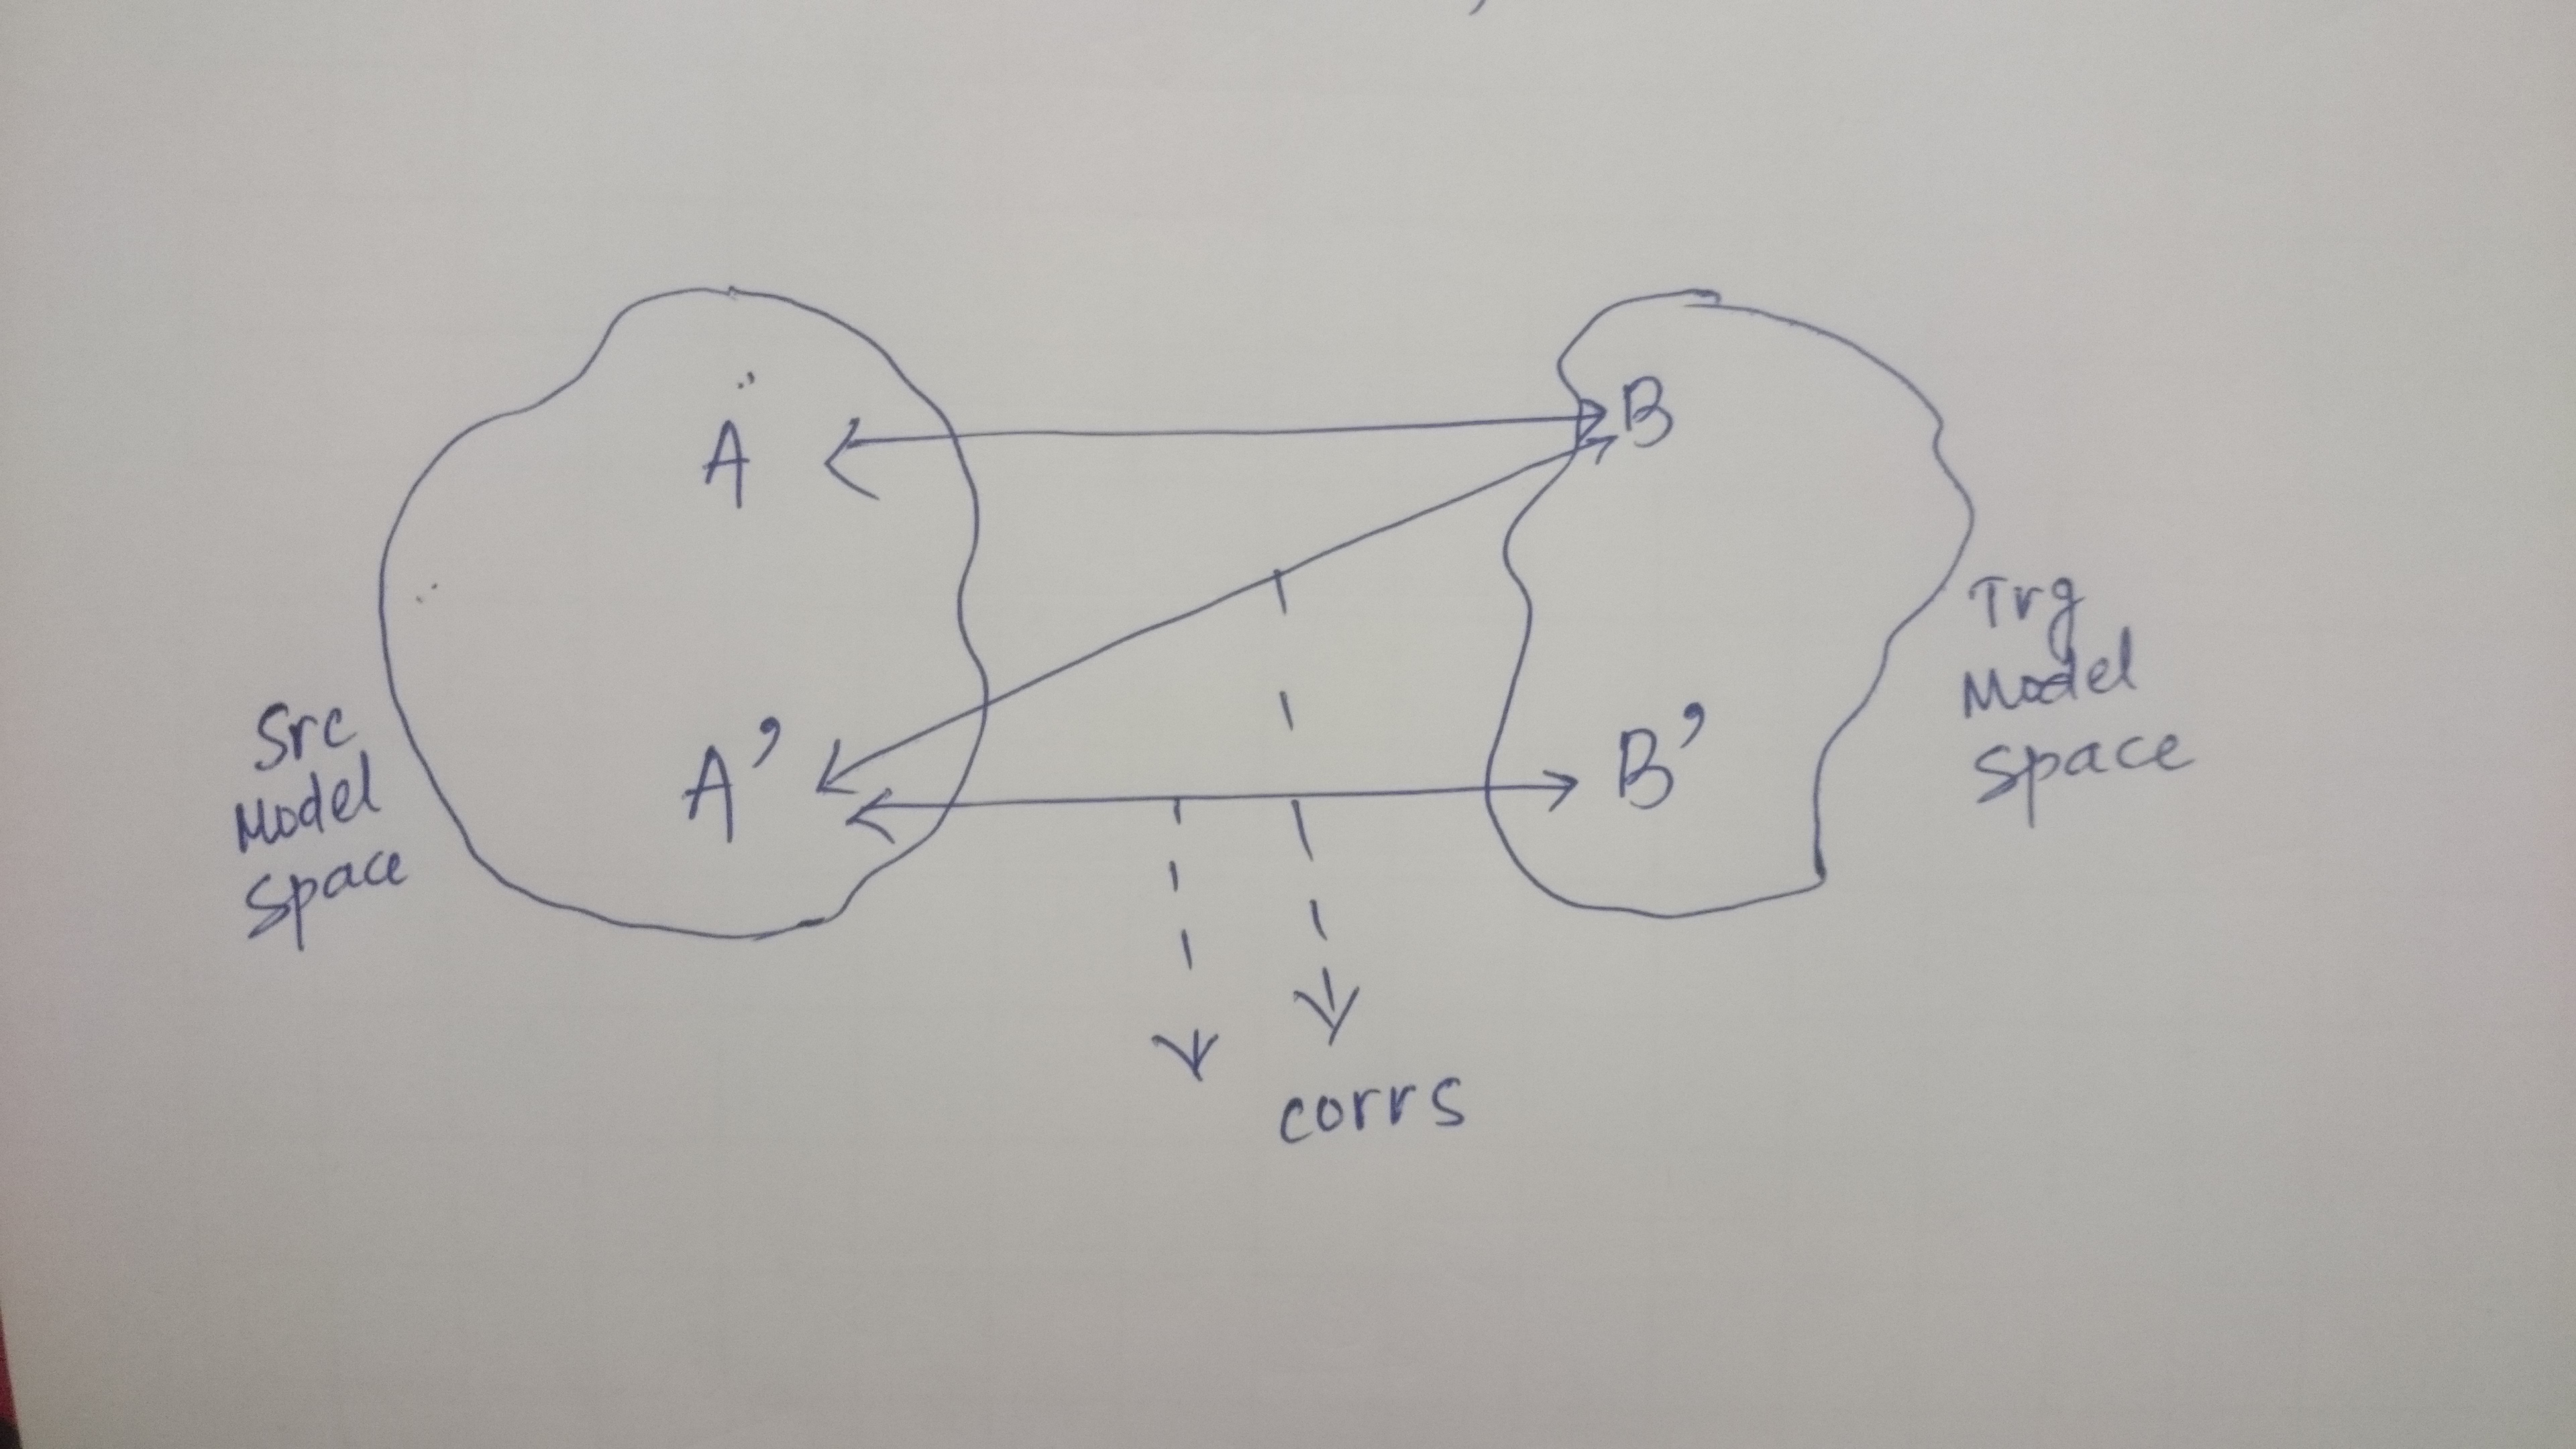
\includegraphics[width=1\textwidth]{figures/Corr}
	\caption{Correspondence Links}
	\label{fig:Correspondence_Links}
\end{figure}

\begin{defn}\label{defConsistency } (Consistency)\\
Changes in one model may or may not cause any change in other model (models from different model spaces) but their states must not contain any contradiction. It is checked on the set of all corrs related to both the models, R: A $\Longleftrightarrow$ B, i.e., the corr R is consistent, or R is inconsistent \cite{benchmarx-reload}.
\end{defn} 

In layman's term, consistent is a state which always involves 2 or more objects/artefacts but doesn't involve ambiguity between them. This is the most important part of the model transformation and the entire focus revolves around it. To be consistent with each other the models have to be inline with respect to their states. 

\textit{Example:} In my demonstrator example, an example of a corr is r(group; itemSocket) where \textit{group}, \textit{itemSocket} are the elements of \textit{Grid} and \textit{Kitchen} Model respectively. Figure~\ref{fig:Running_Example_GUI} and Figure~\ref{fig:Running_Example_GUI_consistency} shows that changes in \textit{Kitchen} model i.e., movement of sink should be propagated to the \textit{Grid} model in order to ensure consistency.\\

\begin{defn}\label{deffwdbkdtrans} (Forward and Backward Transformation)\\
Model transformation is defined as a process for propagating the changes (deltas) from one model of one domain to a corresponding model in another domain using forward and/or backward transformation operations. After a transformation operation, consistency of source and target model is always ensured as model transformation ensures that for each consistent source model there exist a consistent target model~\cite{modelsynchro-tgg}.

In forward transformation, only the changes that occur in the source model is propagated to the target model ensuring the consistency between source and target model.

In backward transformation, only the changes that occur in the target model is propagated to the source model ensuring the consistency between source and target model.

Given two models, bidirectional transformation is a pair of transformation which takes place in both forward and backward direction ensuring the consistency relation between them~\cite{understanding-bx}.

\end{defn}

\textit{Example:} In my demonstrator example, figure~\ref{fig:BX_Diagram} shows an abstract example of the "BX" and figure~\ref{fig:Transformation_Concrete} depicts a concrete example of the "BX" process where a \textit{Grid} model and a \textit{Kitchen} model is described as source and target respectively in the process of forward and backward transformation.

\textit{Example:} In my demonstrator example, "Grid Model" is the \textit{Source} model and "Kitchen Model" is the \textit{Target} model. Forward transformation will cause "Grid Model" to transform into "Kitchen Model" and Backward transformation will cause "Kitchen Model" to transform into "Grid Model". Figure~\ref{fig:Transformation_Abstract} shows an abstract example of the transformation process and figure~\ref{fig:Transformation_Concrete} depicts a concrete example of the transformation process describing both forward and backward transformation.\\

\begin{figure}
	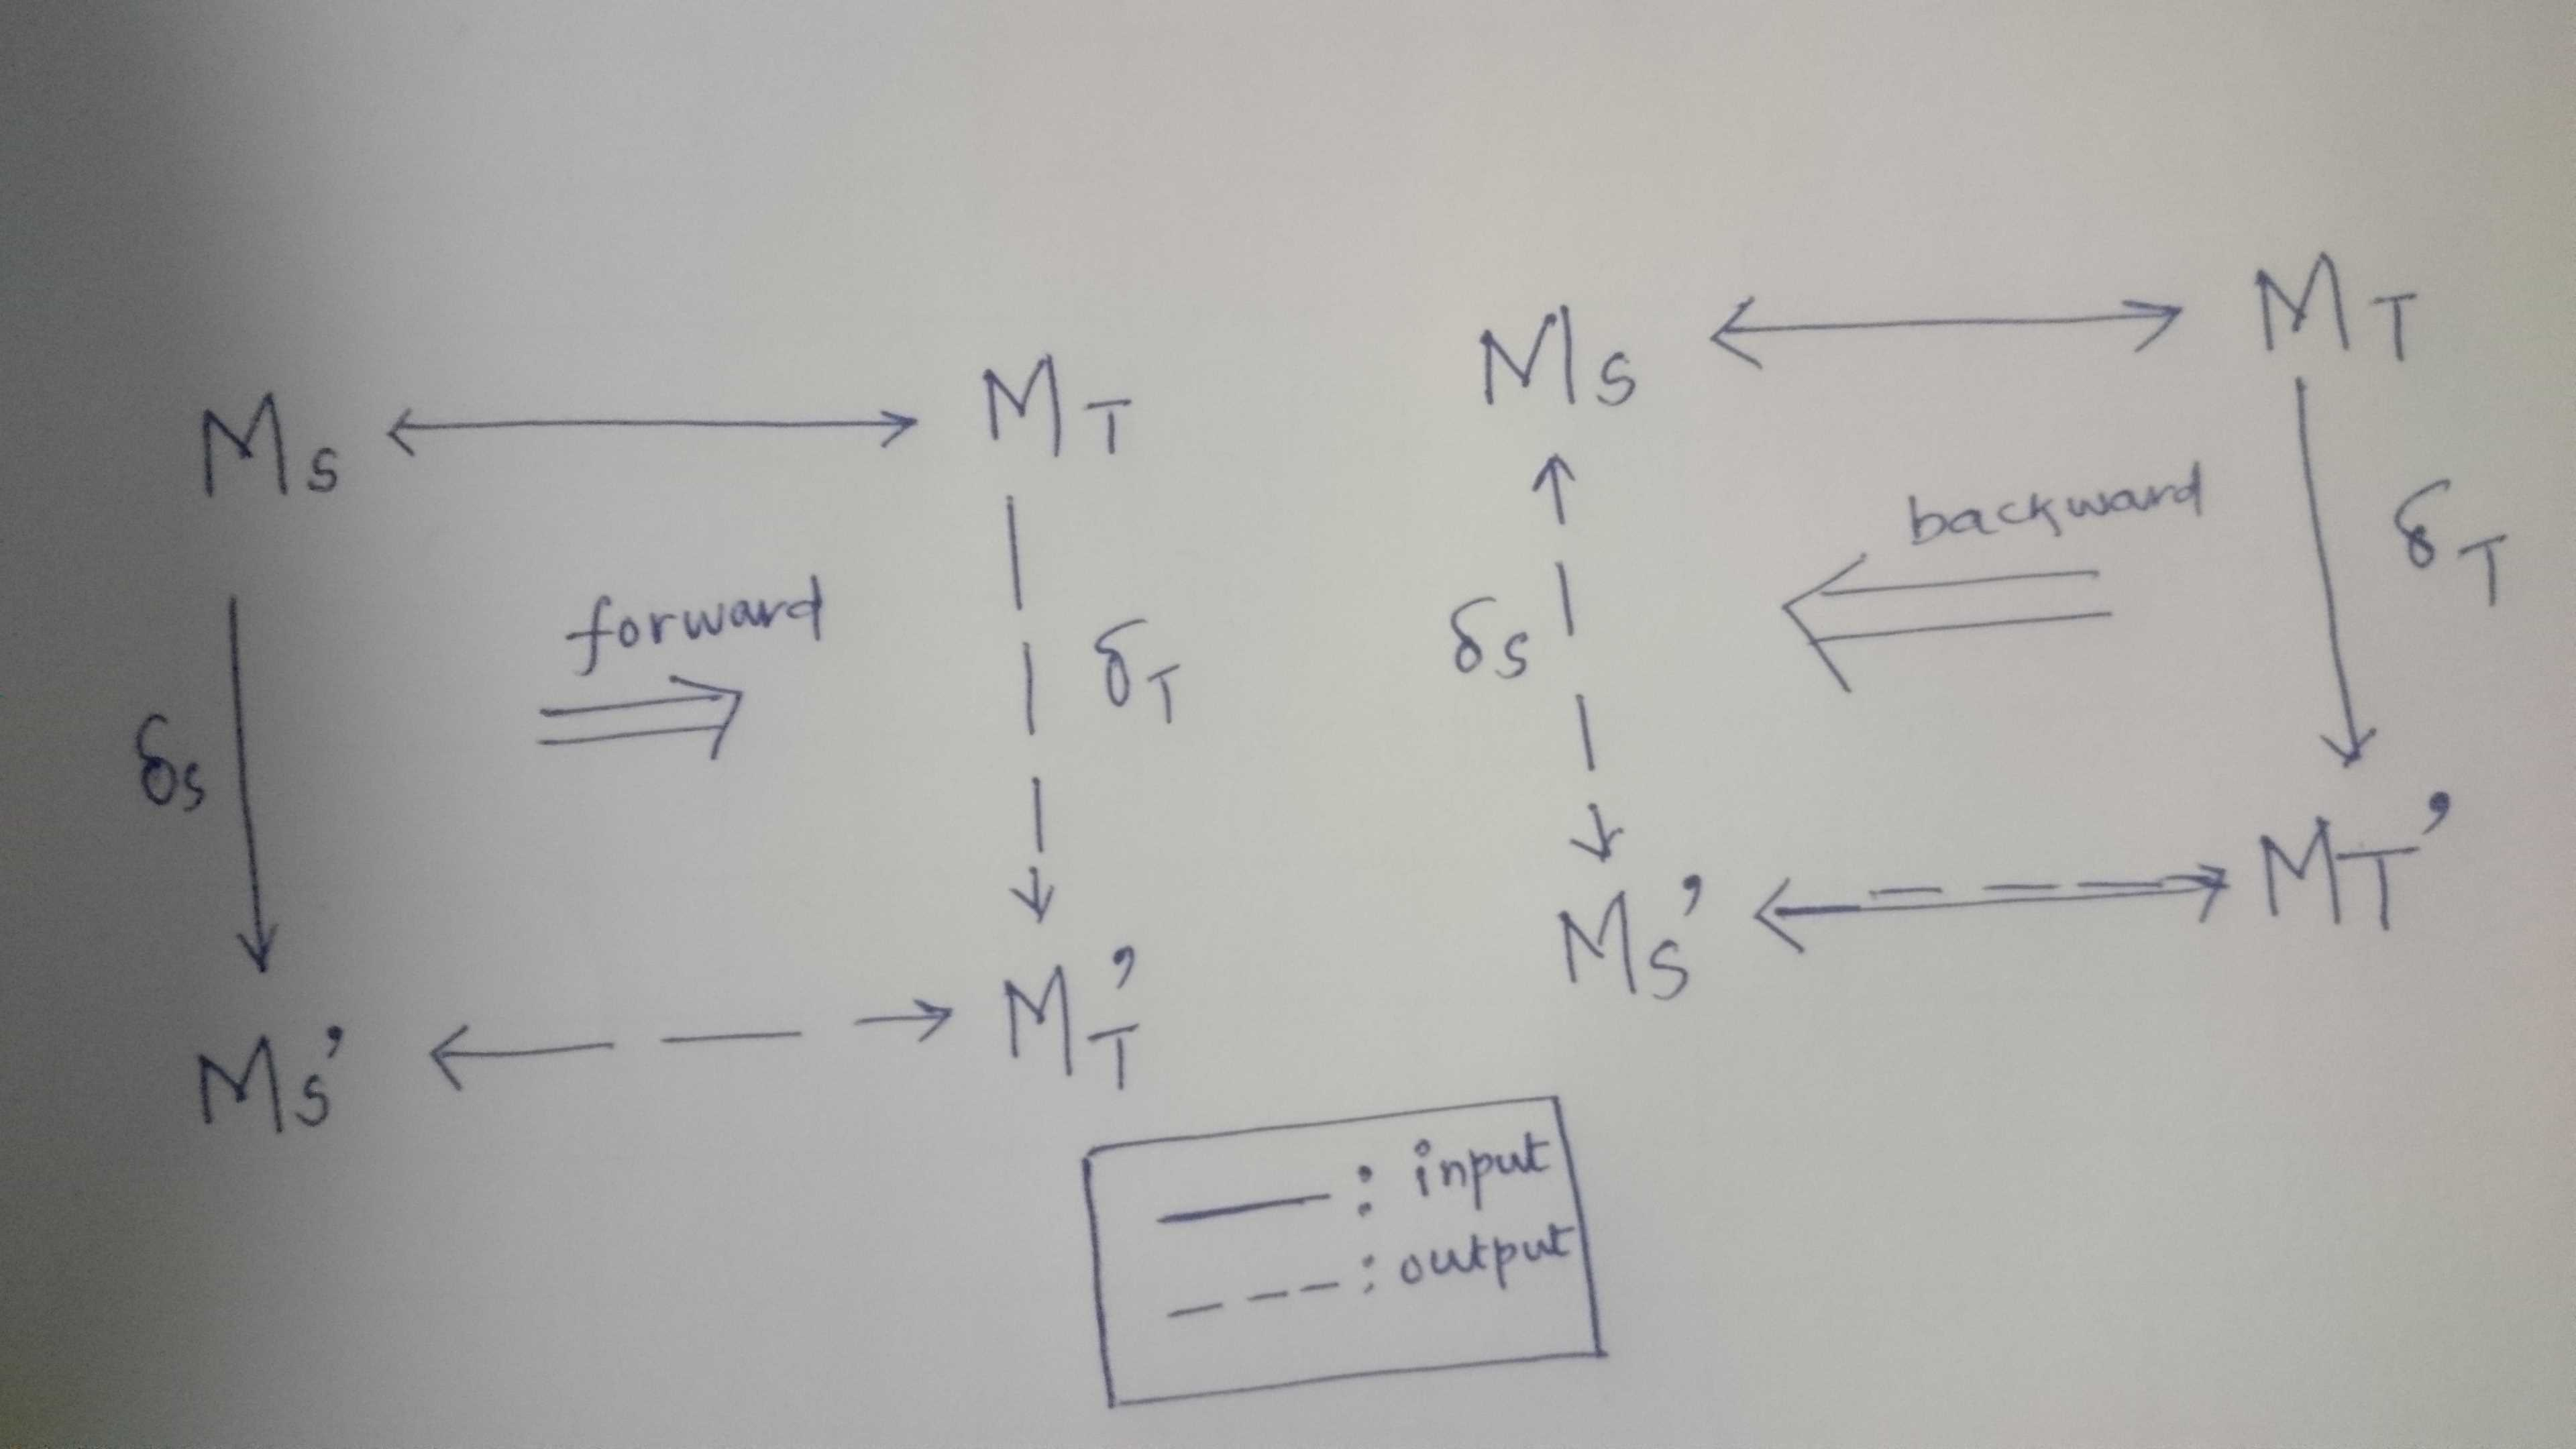
\includegraphics[width=1\textwidth]{figures/BX}
	\caption{Bidirectional Transformation}
	\label{fig:BX_Diagram}
\end{figure}

\begin{figure}
	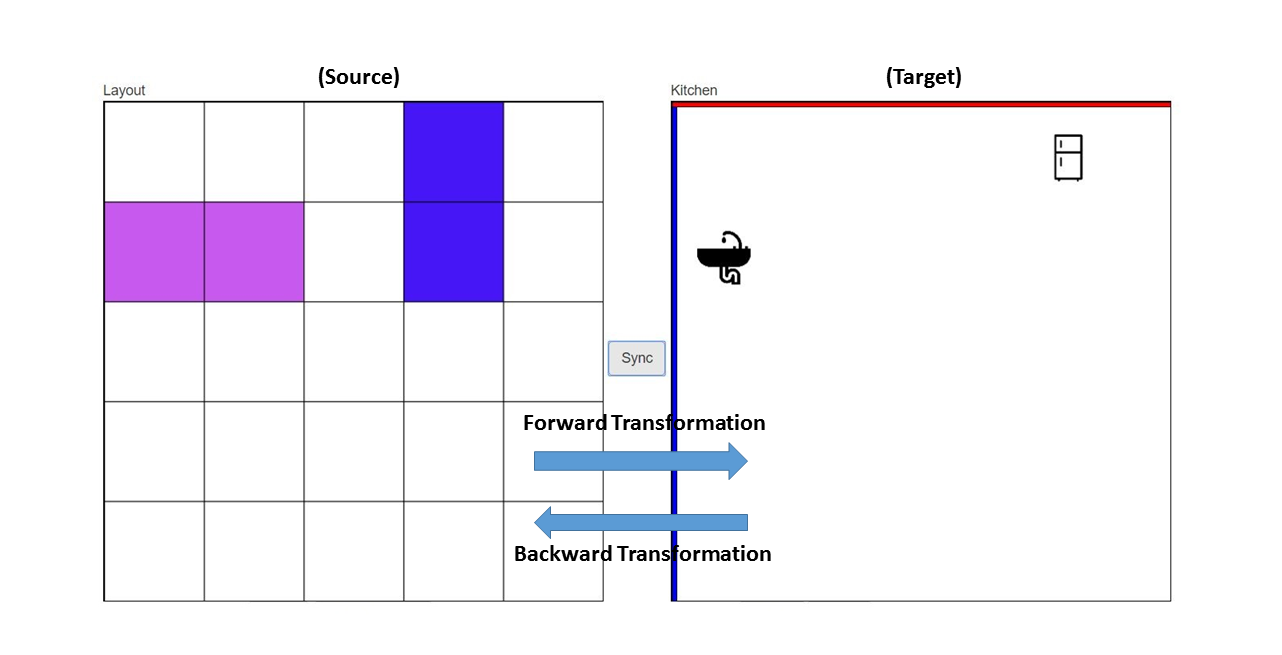
\includegraphics[width=1\textwidth]{figures/Transformation_Concrete}
	\caption{Transformation (Concrete Diagram)}
	\label{fig:Transformation_Concrete}
\end{figure}